%%%%%%%%%%%%%%%%%%%%%%%%%%%%%%%%%%%%%%%%%%%%%%%%%%%%%%%%%%%%%%%%%%%%%%%%
% Escuela Politécnica Superior de la Universidad de Alicante
% Realizado por: Jose Manuel Requena Plens
% Contacto: info@jmrplens.com / Telegram:@jmrplens
%%%%%%%%%%%%%%%%%%%%%%%%%%%%%%%%%%%%%%%%%%%%%%%%%%%%%%%%%%%%%%%%%%%%%%%%

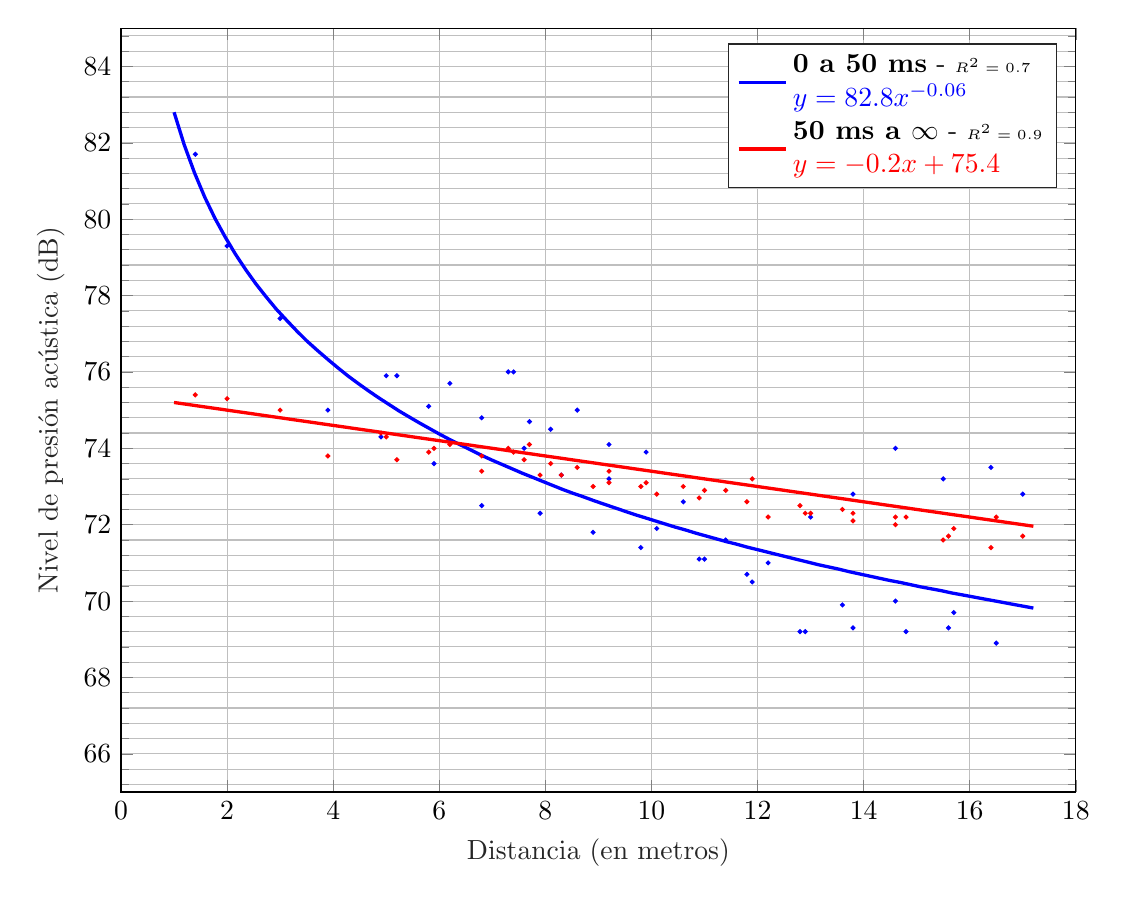
\begin{tikzpicture}

\begin{axis}[%
width=\textwidth,
height=0.8\textwidth,
at={(0\textwidth,0\textwidth)},
scale only axis,
xmin=0,
xmax=18,
xlabel style={font=\color{white!15!black}},
xlabel={Distancia (en metros)},
ymin=65,
ymax=85,
xmajorgrids,
xminorgrids,
ymajorgrids,
yminorgrids,
minor y tick num= 4,
ylabel style={font=\color{white!15!black}},
ylabel={Nivel de presión acústica (dB)},
axis background/.style={fill=white},
%xmajorgrids,
%xminorgrids,
%ymajorgrids,
%yminorgrids,
legend style={legend cell align=left, align=left, draw=white!15!black}
]
\addplot[color=blue,domain=1:17.2, samples=85,line width=1.2]{82.80*x^(-0.06)};
\addlegendentry{\textbf{0 a 50 ms} - \tiny{$R^2 = 0.7$}\\$\color{blue}y = 82.8·x^{-0.06}$}

\addplot[color=red,domain=1:17.2, samples=85, line width=1.2]{-0.2*x+75.4};
\addlegendentry{\textbf{50 ms a $\infty$} - \tiny{$R^2 = 0.9$}\\$\color{red}y = -0.2·x+75.4$}

% Puntos
\addplot [color=blue, only marks,mark size=0.7pt]
  table[row sep=crcr]{%
1.4		81.7\\
2		79.3\\
3		77.4\\
3.9		75\\
4.9		74.3\\
5.9		73.6\\
6.8	72.5\\
7.9	72.3\\
8.9	71.8\\
9.8	71.4\\
10.9	71.1\\
11.8	70.7\\
12.9	69.2\\
13.8	69.3\\
14.8	69.2\\
15.7	69.7\\
5.0	75.9\\
5.2	75.9\\
5.8	75.1\\
6.2	75.7\\
6.8	74.8\\
7.6	74.0\\
8.3	73.3\\
9.2	73.2\\
10.1	71.9\\
11.0	71.1\\
11.9	70.5\\
12.8	69.2\\
13.6	69.9\\
14.6	70.0\\
15.6	69.3\\
16.5	68.9\\
7.3	76.0\\
7.4	76.0\\
7.7	74.7\\
8.1	74.5\\
8.6	75.0\\
9.2	74.1\\
9.9	73.9\\
10.6	72.6\\
11.4	71.6\\
12.2	71.0\\
13.0	72.2\\
13.8	72.8\\
14.6	74.0\\
15.5	73.2\\
16.4	73.5\\
17.0	72.8\\
};

\addplot [color=red, only marks,mark size=0.7pt]
  table[row sep=crcr]{%
  1.4	75.4\\
2.0	75.3\\
3.0	75.0\\
3.9	73.8\\
4.9	74.4\\
5.9	74.0\\
6.8	73.8\\
7.9	73.3\\
8.9	73.0\\
9.8	73.0\\
10.9	72.7\\
11.8	72.6\\
12.9	72.3\\
13.8	72.1\\
14.8	72.2\\
15.7	71.9\\
5.0	74.3\\
5.2	73.7\\
5.8	73.9\\
6.2	74.1\\
6.8	73.4\\
7.6	73.7\\
8.3	73.3\\
9.2	73.1\\
10.1	72.8\\
11.0	72.9\\
11.9	73.2\\
12.8	72.5\\
13.6	72.4\\
14.6	72.2\\
15.6	71.7\\
16.5	72.2\\
7.3	74.0\\
7.4	73.9\\
7.7	74.1\\
8.1	73.6\\
8.6	73.5\\
9.2	73.4\\
9.9	73.1\\
10.6	73.0\\
11.4	72.9\\
12.2	72.2\\
13.0	72.3\\
13.8	72.3\\
14.6	72.0\\
15.5	71.6\\
16.4	71.4\\
17.0	71.7\\
  };
\end{axis}
\end{tikzpicture}%